\documentclass[twoside]{book}

% Packages required by doxygen
\usepackage{fixltx2e}
\usepackage{calc}
\usepackage{doxygen}
\usepackage[export]{adjustbox} % also loads graphicx
\usepackage{graphicx}
\usepackage[utf8]{inputenc}
\usepackage{makeidx}
\usepackage{multicol}
\usepackage{multirow}
\PassOptionsToPackage{warn}{textcomp}
\usepackage{textcomp}
\usepackage[nointegrals]{wasysym}
\usepackage[table]{xcolor}

% Font selection
\usepackage[T1]{fontenc}
\usepackage[scaled=.90]{helvet}
\usepackage{courier}
\usepackage{amssymb}
\usepackage{sectsty}
\renewcommand{\familydefault}{\sfdefault}
\allsectionsfont{%
  \fontseries{bc}\selectfont%
  \color{darkgray}%
}
\renewcommand{\DoxyLabelFont}{%
  \fontseries{bc}\selectfont%
  \color{darkgray}%
}
\newcommand{\+}{\discretionary{\mbox{\scriptsize$\hookleftarrow$}}{}{}}

% Page & text layout
\usepackage{geometry}
\geometry{%
  a4paper,%
  top=2.5cm,%
  bottom=2.5cm,%
  left=2.5cm,%
  right=2.5cm%
}
\tolerance=750
\hfuzz=15pt
\hbadness=750
\setlength{\emergencystretch}{15pt}
\setlength{\parindent}{0cm}
\setlength{\parskip}{3ex plus 2ex minus 2ex}
\makeatletter
\renewcommand{\paragraph}{%
  \@startsection{paragraph}{4}{0ex}{-1.0ex}{1.0ex}{%
    \normalfont\normalsize\bfseries\SS@parafont%
  }%
}
\renewcommand{\subparagraph}{%
  \@startsection{subparagraph}{5}{0ex}{-1.0ex}{1.0ex}{%
    \normalfont\normalsize\bfseries\SS@subparafont%
  }%
}
\makeatother

% Headers & footers
\usepackage{fancyhdr}
\pagestyle{fancyplain}
\fancyhead[LE]{\fancyplain{}{\bfseries\thepage}}
\fancyhead[CE]{\fancyplain{}{}}
\fancyhead[RE]{\fancyplain{}{\bfseries\leftmark}}
\fancyhead[LO]{\fancyplain{}{\bfseries\rightmark}}
\fancyhead[CO]{\fancyplain{}{}}
\fancyhead[RO]{\fancyplain{}{\bfseries\thepage}}
\fancyfoot[LE]{\fancyplain{}{}}
\fancyfoot[CE]{\fancyplain{}{}}
\fancyfoot[RE]{\fancyplain{}{\bfseries\scriptsize Generated by Doxygen }}
\fancyfoot[LO]{\fancyplain{}{\bfseries\scriptsize Generated by Doxygen }}
\fancyfoot[CO]{\fancyplain{}{}}
\fancyfoot[RO]{\fancyplain{}{}}
\renewcommand{\footrulewidth}{0.4pt}
\renewcommand{\chaptermark}[1]{%
  \markboth{#1}{}%
}
\renewcommand{\sectionmark}[1]{%
  \markright{\thesection\ #1}%
}

% Indices & bibliography
\usepackage{natbib}
\usepackage[titles]{tocloft}
\setcounter{tocdepth}{3}
\setcounter{secnumdepth}{5}
\makeindex

% Hyperlinks (required, but should be loaded last)
\usepackage{ifpdf}
\ifpdf
  \usepackage[pdftex,pagebackref=true]{hyperref}
\else
  \usepackage[ps2pdf,pagebackref=true]{hyperref}
\fi
\hypersetup{%
  colorlinks=true,%
  linkcolor=blue,%
  citecolor=blue,%
  unicode%
}

% Custom commands
\newcommand{\clearemptydoublepage}{%
  \newpage{\pagestyle{empty}\cleardoublepage}%
}

\usepackage{caption}
\captionsetup{labelsep=space,justification=centering,font={bf},singlelinecheck=off,skip=4pt,position=top}

%===== C O N T E N T S =====

\begin{document}

% Titlepage & ToC
\hypersetup{pageanchor=false,
             bookmarksnumbered=true,
             pdfencoding=unicode
            }
\pagenumbering{alph}
\begin{titlepage}
\vspace*{7cm}
\begin{center}%
{\Large My Project }\\
\vspace*{1cm}
{\large Generated by Doxygen 1.8.13}\\
\end{center}
\end{titlepage}
\clearemptydoublepage
\pagenumbering{roman}
\tableofcontents
\clearemptydoublepage
\pagenumbering{arabic}
\hypersetup{pageanchor=true}

%--- Begin generated contents ---
\chapter{Namespace Index}
\section{Packages}
Here are the packages with brief descriptions (if available)\+:\begin{DoxyCompactList}
\item\contentsline{section}{\hyperlink{namespace_mail_storage}{Mail\+Storage} }{\pageref{namespace_mail_storage}}{}
\end{DoxyCompactList}

\chapter{Hierarchical Index}
\section{Class Hierarchy}
This inheritance list is sorted roughly, but not completely, alphabetically\+:\begin{DoxyCompactList}
\item \contentsline{section}{Mail\+Storage.\+App\+File}{\pageref{class_mail_storage_1_1_app_file}}{}
\item \contentsline{section}{Mail\+Storage.\+Db\+Manager}{\pageref{class_mail_storage_1_1_db_manager}}{}
\item Form\begin{DoxyCompactList}
\item \contentsline{section}{Mail\+Storage.\+Login\+Window}{\pageref{class_mail_storage_1_1_login_window}}{}
\item \contentsline{section}{Mail\+Storage.\+Mail\+Storage}{\pageref{class_mail_storage_1_1_mail_storage}}{}
\end{DoxyCompactList}
\end{DoxyCompactList}

\chapter{Class Index}
\section{Class List}
Here are the classes, structs, unions and interfaces with brief descriptions\+:\begin{DoxyCompactList}
\item\contentsline{section}{\hyperlink{class_mail_storage_1_1_app_file}{Mail\+Storage.\+App\+File} \\*Files used in the app }{\pageref{class_mail_storage_1_1_app_file}}{}
\item\contentsline{section}{\hyperlink{class_mail_storage_1_1_db_manager}{Mail\+Storage.\+Db\+Manager} \\*Manages all the interaction with the S\+Q\+Lite database }{\pageref{class_mail_storage_1_1_db_manager}}{}
\item\contentsline{section}{\hyperlink{class_mail_storage_1_1_login_window}{Mail\+Storage.\+Login\+Window} \\*The window main class }{\pageref{class_mail_storage_1_1_login_window}}{}
\item\contentsline{section}{\hyperlink{class_mail_storage_1_1_mail_storage}{Mail\+Storage.\+Mail\+Storage} \\*The window main class }{\pageref{class_mail_storage_1_1_mail_storage}}{}
\end{DoxyCompactList}

\chapter{Namespace Documentation}
\hypertarget{namespace_mail_storage}{}\section{Mail\+Storage Namespace Reference}
\label{namespace_mail_storage}\index{Mail\+Storage@{Mail\+Storage}}
\subsection*{Classes}
\begin{DoxyCompactItemize}
\item 
class \hyperlink{class_mail_storage_1_1_app_file}{App\+File}
\begin{DoxyCompactList}\small\item\em Files used in the app \end{DoxyCompactList}\item 
class \hyperlink{class_mail_storage_1_1_db_manager}{Db\+Manager}
\begin{DoxyCompactList}\small\item\em Manages all the interaction with the S\+Q\+Lite database \end{DoxyCompactList}\item 
class {\bfseries Files\+Manager}
\begin{DoxyCompactList}\small\item\em Contains all the functions used to manages the files \end{DoxyCompactList}\item 
class {\bfseries Globals}
\begin{DoxyCompactList}\small\item\em Here are all the program globals and constans \end{DoxyCompactList}\item 
class \hyperlink{class_mail_storage_1_1_login_window}{Login\+Window}
\begin{DoxyCompactList}\small\item\em The window main class \end{DoxyCompactList}\item 
class {\bfseries Mail\+Manager}
\begin{DoxyCompactList}\small\item\em This class manages all the user mailbox interactions and connections \end{DoxyCompactList}\item 
class \hyperlink{class_mail_storage_1_1_mail_storage}{Mail\+Storage}
\begin{DoxyCompactList}\small\item\em The window main class \end{DoxyCompactList}\item 
class {\bfseries Program}
\end{DoxyCompactItemize}

\chapter{Class Documentation}
\hypertarget{class_mail_storage_1_1_app_file}{}\section{Mail\+Storage.\+App\+File Class Reference}
\label{class_mail_storage_1_1_app_file}\index{Mail\+Storage.\+App\+File@{Mail\+Storage.\+App\+File}}


Files used in the app  


\subsection*{Public Member Functions}
\begin{DoxyCompactItemize}
\item 
\hyperlink{class_mail_storage_1_1_app_file_a7d30bfd52976376bf98a71d7f0f2941d}{App\+File} (string str\+File\+Name, string str\+File\+Path, Date\+Time dt\+Creation\+Date, Date\+Time dt\+Modification\+Date)
\begin{DoxyCompactList}\small\item\em Class constructor, creates the file \end{DoxyCompactList}\end{DoxyCompactItemize}
\subsection*{Public Attributes}
\begin{DoxyCompactItemize}
\item 
\mbox{\Hypertarget{class_mail_storage_1_1_app_file_a3181bcb2f55c1e643b00b7b4584b8ed8}\label{class_mail_storage_1_1_app_file_a3181bcb2f55c1e643b00b7b4584b8ed8}} 
string {\bfseries file\+Name}
\item 
\mbox{\Hypertarget{class_mail_storage_1_1_app_file_a5b11dbe8241895ece9e3858b46e53d5a}\label{class_mail_storage_1_1_app_file_a5b11dbe8241895ece9e3858b46e53d5a}} 
string {\bfseries file\+Path}
\item 
\mbox{\Hypertarget{class_mail_storage_1_1_app_file_ad293ee96f042c3b06bf60901b86b7421}\label{class_mail_storage_1_1_app_file_ad293ee96f042c3b06bf60901b86b7421}} 
Date\+Time {\bfseries file\+Creation\+Date}
\item 
\mbox{\Hypertarget{class_mail_storage_1_1_app_file_a80115409ccdda1de48224beb8c1c22dc}\label{class_mail_storage_1_1_app_file_a80115409ccdda1de48224beb8c1c22dc}} 
Date\+Time {\bfseries file\+Modification\+Date}
\end{DoxyCompactItemize}


\subsection{Detailed Description}
Files used in the app 



\subsection{Constructor \& Destructor Documentation}
\mbox{\Hypertarget{class_mail_storage_1_1_app_file_a7d30bfd52976376bf98a71d7f0f2941d}\label{class_mail_storage_1_1_app_file_a7d30bfd52976376bf98a71d7f0f2941d}} 
\index{Mail\+Storage\+::\+App\+File@{Mail\+Storage\+::\+App\+File}!App\+File@{App\+File}}
\index{App\+File@{App\+File}!Mail\+Storage\+::\+App\+File@{Mail\+Storage\+::\+App\+File}}
\subsubsection{\texorpdfstring{App\+File()}{AppFile()}}
{\footnotesize\ttfamily Mail\+Storage.\+App\+File.\+App\+File (\begin{DoxyParamCaption}\item[{string}]{str\+File\+Name,  }\item[{string}]{str\+File\+Path,  }\item[{Date\+Time}]{dt\+Creation\+Date,  }\item[{Date\+Time}]{dt\+Modification\+Date }\end{DoxyParamCaption})}



Class constructor, creates the file 



The documentation for this class was generated from the following file\+:\begin{DoxyCompactItemize}
\item 
App\+File.\+cs\end{DoxyCompactItemize}

\hypertarget{class_mail_storage_1_1_db_manager}{}\section{Mail\+Storage.\+Db\+Manager Class Reference}
\label{class_mail_storage_1_1_db_manager}\index{Mail\+Storage.\+Db\+Manager@{Mail\+Storage.\+Db\+Manager}}


Manages all the interaction with the S\+Q\+Lite database  


\subsection*{Public Member Functions}
\begin{DoxyCompactItemize}
\item 
\hyperlink{class_mail_storage_1_1_db_manager_a2fce4fc8a19fd0f0de40091d2dc96931}{Db\+Manager} ()
\begin{DoxyCompactList}\small\item\em Class constructor, creates the database if it doesn\textquotesingle{}t exist \end{DoxyCompactList}\item 
void \hyperlink{class_mail_storage_1_1_db_manager_a862704b090f1a99e33682f701c6f8ba2}{Update\+User\+Data} (string server\+Name, string server\+Port, string user\+Mail, string user\+Password, string dir\+Path)
\begin{DoxyCompactList}\small\item\em Inserts all the data into the database \end{DoxyCompactList}\item 
List$<$ string $>$ \hyperlink{class_mail_storage_1_1_db_manager_add360de0a5bb47870412e69741da22f3}{Get\+Current\+User\+Data} ()
\begin{DoxyCompactList}\small\item\em Gets the registered user from the database \end{DoxyCompactList}\end{DoxyCompactItemize}


\subsection{Detailed Description}
Manages all the interaction with the S\+Q\+Lite database 



\subsection{Constructor \& Destructor Documentation}
\mbox{\Hypertarget{class_mail_storage_1_1_db_manager_a2fce4fc8a19fd0f0de40091d2dc96931}\label{class_mail_storage_1_1_db_manager_a2fce4fc8a19fd0f0de40091d2dc96931}} 
\index{Mail\+Storage\+::\+Db\+Manager@{Mail\+Storage\+::\+Db\+Manager}!Db\+Manager@{Db\+Manager}}
\index{Db\+Manager@{Db\+Manager}!Mail\+Storage\+::\+Db\+Manager@{Mail\+Storage\+::\+Db\+Manager}}
\subsubsection{\texorpdfstring{Db\+Manager()}{DbManager()}}
{\footnotesize\ttfamily Mail\+Storage.\+Db\+Manager.\+Db\+Manager (\begin{DoxyParamCaption}{ }\end{DoxyParamCaption})}



Class constructor, creates the database if it doesn\textquotesingle{}t exist 



\subsection{Member Function Documentation}
\mbox{\Hypertarget{class_mail_storage_1_1_db_manager_add360de0a5bb47870412e69741da22f3}\label{class_mail_storage_1_1_db_manager_add360de0a5bb47870412e69741da22f3}} 
\index{Mail\+Storage\+::\+Db\+Manager@{Mail\+Storage\+::\+Db\+Manager}!Get\+Current\+User\+Data@{Get\+Current\+User\+Data}}
\index{Get\+Current\+User\+Data@{Get\+Current\+User\+Data}!Mail\+Storage\+::\+Db\+Manager@{Mail\+Storage\+::\+Db\+Manager}}
\subsubsection{\texorpdfstring{Get\+Current\+User\+Data()}{GetCurrentUserData()}}
{\footnotesize\ttfamily List$<$string$>$ Mail\+Storage.\+Db\+Manager.\+Get\+Current\+User\+Data (\begin{DoxyParamCaption}{ }\end{DoxyParamCaption})}



Gets the registered user from the database 

\begin{DoxyReturn}{Returns}
Returns a list with all the data
\end{DoxyReturn}
\mbox{\Hypertarget{class_mail_storage_1_1_db_manager_a862704b090f1a99e33682f701c6f8ba2}\label{class_mail_storage_1_1_db_manager_a862704b090f1a99e33682f701c6f8ba2}} 
\index{Mail\+Storage\+::\+Db\+Manager@{Mail\+Storage\+::\+Db\+Manager}!Update\+User\+Data@{Update\+User\+Data}}
\index{Update\+User\+Data@{Update\+User\+Data}!Mail\+Storage\+::\+Db\+Manager@{Mail\+Storage\+::\+Db\+Manager}}
\subsubsection{\texorpdfstring{Update\+User\+Data()}{UpdateUserData()}}
{\footnotesize\ttfamily void Mail\+Storage.\+Db\+Manager.\+Update\+User\+Data (\begin{DoxyParamCaption}\item[{string}]{server\+Name,  }\item[{string}]{server\+Port,  }\item[{string}]{user\+Mail,  }\item[{string}]{user\+Password,  }\item[{string}]{dir\+Path }\end{DoxyParamCaption})}



Inserts all the data into the database 


\begin{DoxyParams}{Parameters}
{\em server\+Name} & The I\+M\+AP server name\\
\hline
{\em server\+Port} & The server port\\
\hline
{\em user\+Mail} & The user mail address\\
\hline
{\em user\+Password} & The user password\\
\hline
{\em dir\+Path} & The root directory path\\
\hline
\end{DoxyParams}


The documentation for this class was generated from the following file\+:\begin{DoxyCompactItemize}
\item 
Db\+Manager.\+cs\end{DoxyCompactItemize}

\hypertarget{class_mail_storage_1_1_login_window}{}\section{Mail\+Storage.\+Login\+Window Class Reference}
\label{class_mail_storage_1_1_login_window}\index{Mail\+Storage.\+Login\+Window@{Mail\+Storage.\+Login\+Window}}


The window main class  


Inheritance diagram for Mail\+Storage.\+Login\+Window\+:\begin{figure}[H]
\begin{center}
\leavevmode
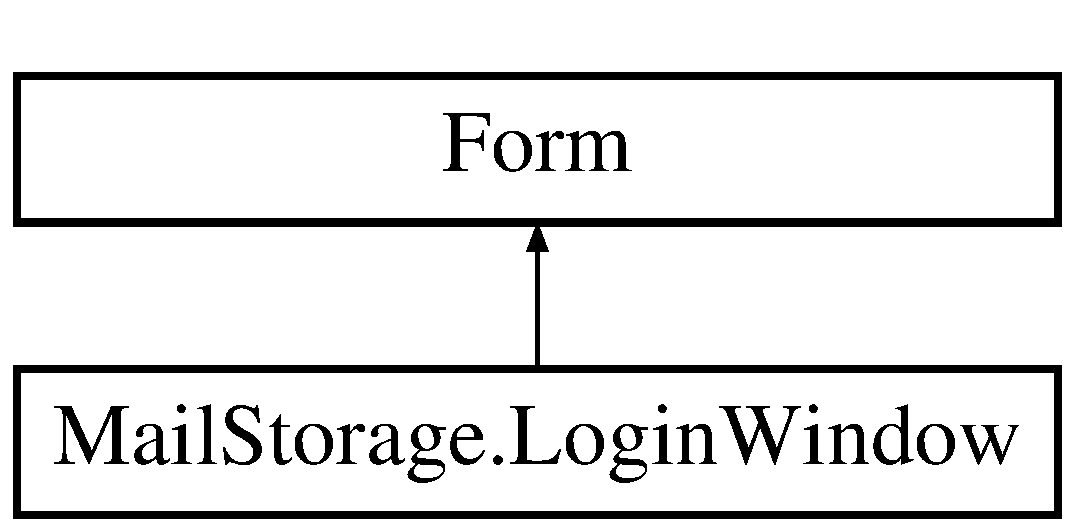
\includegraphics[height=2.000000cm]{class_mail_storage_1_1_login_window}
\end{center}
\end{figure}
\subsection*{Public Member Functions}
\begin{DoxyCompactItemize}
\item 
\mbox{\Hypertarget{class_mail_storage_1_1_login_window_a6b8e304b549a9eb2a38ed2d6375982a2}\label{class_mail_storage_1_1_login_window_a6b8e304b549a9eb2a38ed2d6375982a2}} 
static int {\bfseries Send\+Message} (Int\+Ptr h\+Wnd, int Msg, int w\+Param, int l\+Param)
\item 
\mbox{\Hypertarget{class_mail_storage_1_1_login_window_a47f4a1016d7636c31560a4b315fa14e0}\label{class_mail_storage_1_1_login_window_a47f4a1016d7636c31560a4b315fa14e0}} 
static bool {\bfseries Release\+Capture} ()
\item 
\hyperlink{class_mail_storage_1_1_login_window_a753823a2cafd3253de32a8210d7e0edf}{Login\+Window} ()
\begin{DoxyCompactList}\small\item\em Class constructor \end{DoxyCompactList}\end{DoxyCompactItemize}
\subsection*{Public Attributes}
\begin{DoxyCompactItemize}
\item 
\mbox{\Hypertarget{class_mail_storage_1_1_login_window_a42f7a7d7b8fd211f2f86901863677132}\label{class_mail_storage_1_1_login_window_a42f7a7d7b8fd211f2f86901863677132}} 
const int {\bfseries W\+M\+\_\+\+N\+C\+L\+B\+U\+T\+T\+O\+N\+D\+O\+WN} = 0x\+A1
\item 
\mbox{\Hypertarget{class_mail_storage_1_1_login_window_a96f19a37bb5abefd4e1ac01517f6e751}\label{class_mail_storage_1_1_login_window_a96f19a37bb5abefd4e1ac01517f6e751}} 
const int {\bfseries H\+T\+\_\+\+C\+A\+P\+T\+I\+ON} = 0x2
\end{DoxyCompactItemize}
\subsection*{Protected Member Functions}
\begin{DoxyCompactItemize}
\item 
override void \hyperlink{class_mail_storage_1_1_login_window_a974820001e831196d189c51d64782cfc}{Dispose} (bool disposing)
\begin{DoxyCompactList}\small\item\em Clean up any resources being used. \end{DoxyCompactList}\end{DoxyCompactItemize}


\subsection{Detailed Description}
The window main class 



\subsection{Constructor \& Destructor Documentation}
\mbox{\Hypertarget{class_mail_storage_1_1_login_window_a753823a2cafd3253de32a8210d7e0edf}\label{class_mail_storage_1_1_login_window_a753823a2cafd3253de32a8210d7e0edf}} 
\index{Mail\+Storage\+::\+Login\+Window@{Mail\+Storage\+::\+Login\+Window}!Login\+Window@{Login\+Window}}
\index{Login\+Window@{Login\+Window}!Mail\+Storage\+::\+Login\+Window@{Mail\+Storage\+::\+Login\+Window}}
\subsubsection{\texorpdfstring{Login\+Window()}{LoginWindow()}}
{\footnotesize\ttfamily Mail\+Storage.\+Login\+Window.\+Login\+Window (\begin{DoxyParamCaption}{ }\end{DoxyParamCaption})}



Class constructor 



\subsection{Member Function Documentation}
\mbox{\Hypertarget{class_mail_storage_1_1_login_window_a974820001e831196d189c51d64782cfc}\label{class_mail_storage_1_1_login_window_a974820001e831196d189c51d64782cfc}} 
\index{Mail\+Storage\+::\+Login\+Window@{Mail\+Storage\+::\+Login\+Window}!Dispose@{Dispose}}
\index{Dispose@{Dispose}!Mail\+Storage\+::\+Login\+Window@{Mail\+Storage\+::\+Login\+Window}}
\subsubsection{\texorpdfstring{Dispose()}{Dispose()}}
{\footnotesize\ttfamily override void Mail\+Storage.\+Login\+Window.\+Dispose (\begin{DoxyParamCaption}\item[{bool}]{disposing }\end{DoxyParamCaption})\hspace{0.3cm}{\ttfamily [protected]}}



Clean up any resources being used. 


\begin{DoxyParams}{Parameters}
{\em disposing} & true if managed resources should be disposed; otherwise, false.\\
\hline
\end{DoxyParams}


The documentation for this class was generated from the following files\+:\begin{DoxyCompactItemize}
\item 
Login\+Window.\+cs\item 
Login\+Window.\+Designer.\+cs\end{DoxyCompactItemize}

\hypertarget{class_mail_storage_1_1_mail_storage}{}\section{Mail\+Storage.\+Mail\+Storage Class Reference}
\label{class_mail_storage_1_1_mail_storage}\index{Mail\+Storage.\+Mail\+Storage@{Mail\+Storage.\+Mail\+Storage}}


The window main class  


Inheritance diagram for Mail\+Storage.\+Mail\+Storage\+:\begin{figure}[H]
\begin{center}
\leavevmode
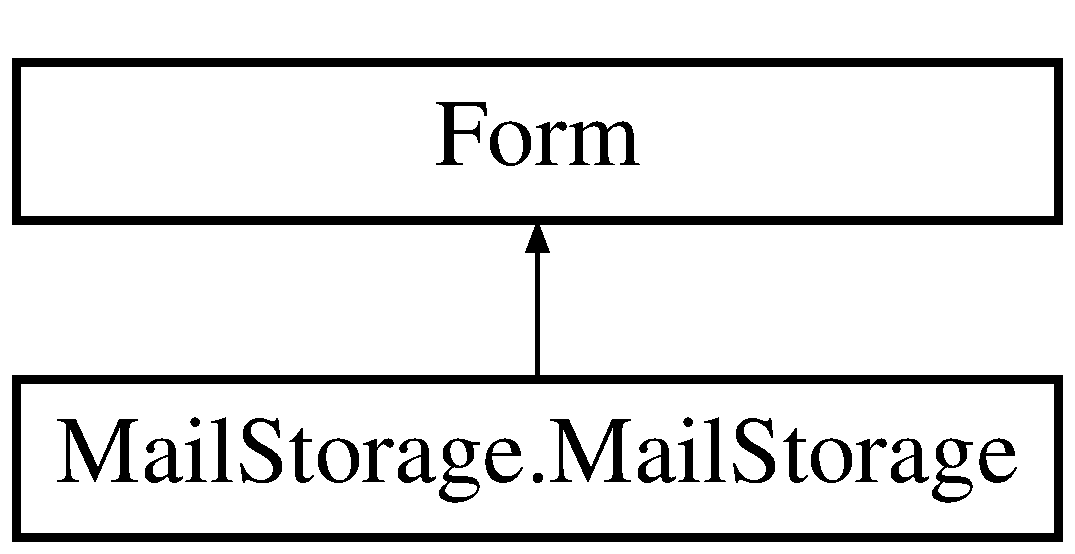
\includegraphics[height=2.000000cm]{class_mail_storage_1_1_mail_storage}
\end{center}
\end{figure}
\subsection*{Public Member Functions}
\begin{DoxyCompactItemize}
\item 
\mbox{\Hypertarget{class_mail_storage_1_1_mail_storage_a57cf4c19f36b8c6cba262eb476ef5a08}\label{class_mail_storage_1_1_mail_storage_a57cf4c19f36b8c6cba262eb476ef5a08}} 
static int {\bfseries Send\+Message} (Int\+Ptr h\+Wnd, int Msg, int w\+Param, int l\+Param)
\item 
\mbox{\Hypertarget{class_mail_storage_1_1_mail_storage_a7a15caac592591ca913d6fb12cf58488}\label{class_mail_storage_1_1_mail_storage_a7a15caac592591ca913d6fb12cf58488}} 
static bool {\bfseries Release\+Capture} ()
\item 
\hyperlink{class_mail_storage_1_1_mail_storage_aa83a233c9413b11ed949ade4a1ed6a23}{Mail\+Storage} ()
\begin{DoxyCompactList}\small\item\em Class constructor \end{DoxyCompactList}\item 
async void \hyperlink{class_mail_storage_1_1_mail_storage_a3be6ac5a1a821602bd40289b48ef34cb}{Initialize\+Window} ()
\begin{DoxyCompactList}\small\item\em Initializes the window when called \end{DoxyCompactList}\item 
void \hyperlink{class_mail_storage_1_1_mail_storage_a6786eea13365af4431e55937b52b8e22}{Update\+Current\+File} (string str\+Text)
\begin{DoxyCompactList}\small\item\em Updates the current file status label \end{DoxyCompactList}\end{DoxyCompactItemize}
\subsection*{Public Attributes}
\begin{DoxyCompactItemize}
\item 
\mbox{\Hypertarget{class_mail_storage_1_1_mail_storage_a18b7c003fb2e0224c49170ce3860b776}\label{class_mail_storage_1_1_mail_storage_a18b7c003fb2e0224c49170ce3860b776}} 
const int {\bfseries W\+M\+\_\+\+N\+C\+L\+B\+U\+T\+T\+O\+N\+D\+O\+WN} = 0x\+A1
\item 
\mbox{\Hypertarget{class_mail_storage_1_1_mail_storage_a2fda94acfe6689309e7a686d80df2282}\label{class_mail_storage_1_1_mail_storage_a2fda94acfe6689309e7a686d80df2282}} 
const int {\bfseries H\+T\+\_\+\+C\+A\+P\+T\+I\+ON} = 0x2
\item 
\mbox{\Hypertarget{class_mail_storage_1_1_mail_storage_a67aceb1c37ff2921d1263c5a3d5ad256}\label{class_mail_storage_1_1_mail_storage_a67aceb1c37ff2921d1263c5a3d5ad256}} 
Task {\bfseries initial\+Sync}
\item 
\mbox{\Hypertarget{class_mail_storage_1_1_mail_storage_ab06602e92c2881e496b03852e2732729}\label{class_mail_storage_1_1_mail_storage_ab06602e92c2881e496b03852e2732729}} 
Task {\bfseries global\+Refresh}
\item 
\mbox{\Hypertarget{class_mail_storage_1_1_mail_storage_a9b813f6d46a8e4d5ac8103648a161a0c}\label{class_mail_storage_1_1_mail_storage_a9b813f6d46a8e4d5ac8103648a161a0c}} 
Task {\bfseries get\+Quota}
\end{DoxyCompactItemize}
\subsection*{Protected Member Functions}
\begin{DoxyCompactItemize}
\item 
override void \hyperlink{class_mail_storage_1_1_mail_storage_a08abad1b434fac866b442755bed1c9f8}{Dispose} (bool disposing)
\begin{DoxyCompactList}\small\item\em Nettoyage des ressources utilisées. \end{DoxyCompactList}\end{DoxyCompactItemize}


\subsection{Detailed Description}
The window main class 



\subsection{Constructor \& Destructor Documentation}
\mbox{\Hypertarget{class_mail_storage_1_1_mail_storage_aa83a233c9413b11ed949ade4a1ed6a23}\label{class_mail_storage_1_1_mail_storage_aa83a233c9413b11ed949ade4a1ed6a23}} 
\index{Mail\+Storage\+::\+Mail\+Storage@{Mail\+Storage\+::\+Mail\+Storage}!Mail\+Storage@{Mail\+Storage}}
\index{Mail\+Storage@{Mail\+Storage}!Mail\+Storage\+::\+Mail\+Storage@{Mail\+Storage\+::\+Mail\+Storage}}
\subsubsection{\texorpdfstring{Mail\+Storage()}{MailStorage()}}
{\footnotesize\ttfamily Mail\+Storage.\+Mail\+Storage.\+Mail\+Storage (\begin{DoxyParamCaption}{ }\end{DoxyParamCaption})}



Class constructor 



\subsection{Member Function Documentation}
\mbox{\Hypertarget{class_mail_storage_1_1_mail_storage_a08abad1b434fac866b442755bed1c9f8}\label{class_mail_storage_1_1_mail_storage_a08abad1b434fac866b442755bed1c9f8}} 
\index{Mail\+Storage\+::\+Mail\+Storage@{Mail\+Storage\+::\+Mail\+Storage}!Dispose@{Dispose}}
\index{Dispose@{Dispose}!Mail\+Storage\+::\+Mail\+Storage@{Mail\+Storage\+::\+Mail\+Storage}}
\subsubsection{\texorpdfstring{Dispose()}{Dispose()}}
{\footnotesize\ttfamily override void Mail\+Storage.\+Mail\+Storage.\+Dispose (\begin{DoxyParamCaption}\item[{bool}]{disposing }\end{DoxyParamCaption})\hspace{0.3cm}{\ttfamily [protected]}}



Nettoyage des ressources utilisées. 


\begin{DoxyParams}{Parameters}
{\em disposing} & true si les ressources managées doivent être supprimées ; sinon, false.\\
\hline
\end{DoxyParams}
\mbox{\Hypertarget{class_mail_storage_1_1_mail_storage_a3be6ac5a1a821602bd40289b48ef34cb}\label{class_mail_storage_1_1_mail_storage_a3be6ac5a1a821602bd40289b48ef34cb}} 
\index{Mail\+Storage\+::\+Mail\+Storage@{Mail\+Storage\+::\+Mail\+Storage}!Initialize\+Window@{Initialize\+Window}}
\index{Initialize\+Window@{Initialize\+Window}!Mail\+Storage\+::\+Mail\+Storage@{Mail\+Storage\+::\+Mail\+Storage}}
\subsubsection{\texorpdfstring{Initialize\+Window()}{InitializeWindow()}}
{\footnotesize\ttfamily async void Mail\+Storage.\+Mail\+Storage.\+Initialize\+Window (\begin{DoxyParamCaption}{ }\end{DoxyParamCaption})}



Initializes the window when called 

\mbox{\Hypertarget{class_mail_storage_1_1_mail_storage_a6786eea13365af4431e55937b52b8e22}\label{class_mail_storage_1_1_mail_storage_a6786eea13365af4431e55937b52b8e22}} 
\index{Mail\+Storage\+::\+Mail\+Storage@{Mail\+Storage\+::\+Mail\+Storage}!Update\+Current\+File@{Update\+Current\+File}}
\index{Update\+Current\+File@{Update\+Current\+File}!Mail\+Storage\+::\+Mail\+Storage@{Mail\+Storage\+::\+Mail\+Storage}}
\subsubsection{\texorpdfstring{Update\+Current\+File()}{UpdateCurrentFile()}}
{\footnotesize\ttfamily void Mail\+Storage.\+Mail\+Storage.\+Update\+Current\+File (\begin{DoxyParamCaption}\item[{string}]{str\+Text }\end{DoxyParamCaption})}



Updates the current file status label 


\begin{DoxyParams}{Parameters}
{\em str\+Text} & \\
\hline
\end{DoxyParams}


The documentation for this class was generated from the following files\+:\begin{DoxyCompactItemize}
\item 
Mail\+Storage.\+cs\item 
Mail\+Storage.\+Designer.\+cs\end{DoxyCompactItemize}

%--- End generated contents ---

% Index
\backmatter
\newpage
\phantomsection
\clearemptydoublepage
\addcontentsline{toc}{chapter}{Index}
\printindex

\end{document}
